%%%%%%%%%%%%%%%%%%%%%%%%%%%%%%%%%%%%%%%%%%%%%%%%%%%%%%%%%%%%%%%%%%%%%%%%%%%

\documentclass{standalone}

\usepackage{amsmath}
\usepackage{mathptmx}
\usepackage{tikz}
\usetikzlibrary{external}
\tikzexternalize{complete-square-a1-c0_halfb}

%% IEEE uses Times Roman font, so we'll default to Times.
%% These three commands make up the entire times.sty package.
\renewcommand{\rmdefault}{ptm}
\renewcommand{\ttdefault}{pcr}
\normalfont\selectfont

%%%%%%%%%%%%%%%%%%%%%%%%%%%%%%%%%%%%%%%%%%%%%%%%%%%%%%%%%%%%%%%%%%%%%%%%%%%
%% Completing the square for the function f(x) = x^2 + bx.
%%%%%%%%%%%%%%%%%%%%%%%%%%%%%%%%%%%%%%%%%%%%%%%%%%%%%%%%%%%%%%%%%%%%%%%%%%%

\begin{document}

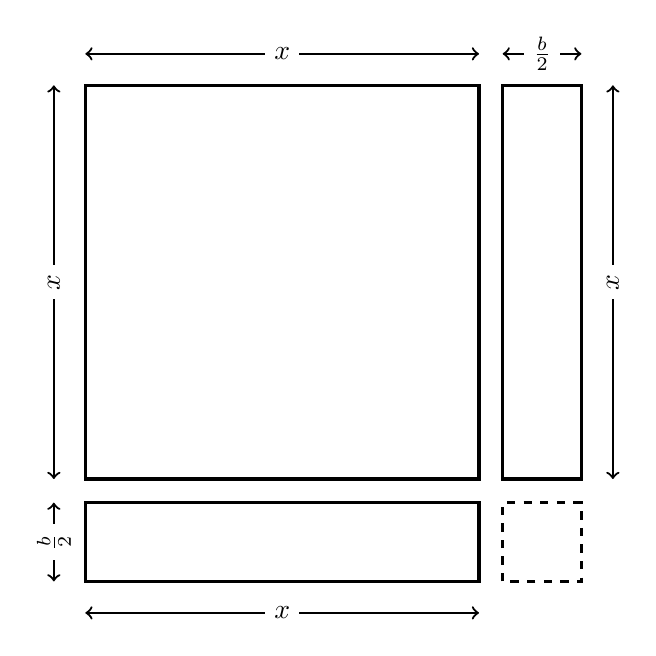
\begin{tikzpicture}[%%
  arrowStyle/.style={<->,thick},%%
  dashStyle/.style={-,dashed,very thick},%%
  labelStyle/.style={fill=white},%%
  lineStyle/.style={-,very thick}%%
]
%%
%%
\pgfmathsetmacro{\bside}{1}  %% width or height of rectangle
\pgfmathsetmacro{\dbx}{0.3}  %% gap between square and rectangle
\pgfmathsetmacro{\dx}{0.4}
\pgfmathsetmacro{\dy}{\dx}
\pgfmathsetmacro{\xlow}{0}
\pgfmathsetmacro{\xside}{5}  %% height of square
\pgfmathsetmacro{\ylow}{\xlow}
%% The right rectangle.
\pgfmathsetmacro{\bxend}{\xside+\dbx+\bside}
\pgfmathsetmacro{\bxstart}{\xside+\dbx}
\pgfmathsetmacro{\byend}{\xside}
\pgfmathsetmacro{\bystart}{\ylow}
%% The bottom rectangle.
\pgfmathsetmacro{\Bxend}{\xside}
\pgfmathsetmacro{\Bxstart}{\xlow}
\pgfmathsetmacro{\Byend}{-\dbx}
\pgfmathsetmacro{\Bystart}{-\dbx-\bside}
%% The dashed square.
\pgfmathsetmacro{\dxend}{\Bxend+\dbx+\bside}
\pgfmathsetmacro{\dxstart}{\Bxend+\dbx}
\pgfmathsetmacro{\dyend}{-\dbx}
\pgfmathsetmacro{\dystart}{-\dbx-\bside}
%%
%% Coordinates for the square.
\coordinate (xlowerLeft) at (\xlow,\ylow);
\coordinate (xupperRight) at (\xside,\xside);
%% Coordinates for the right rectangle.
\coordinate (blowerLeft) at (\bxstart,\bystart);
\coordinate (bupperRight) at (\bxend,\byend);
%% Coordinates for the bottom rectangle.
\coordinate (BlowerLeft) at (\Bxstart,\Bystart);
\coordinate (BupperRight) at (\Bxend,\Byend);
%% Coordinates for the dashed square.
\coordinate (dlowerLeft) at (\dxstart,\dystart);
\coordinate (dupperRight) at (\dxend,\dyend);
%%
\normalsize
%% Draw and label the square.
%% Draw the square.
\draw[lineStyle] (xlowerLeft) rectangle (xupperRight);
%% Label the length of the square.
\draw[arrowStyle] (\xlow,\xside+\dx) -- (\xside,\xside+\dx);
\node[labelStyle] at (\xside/2,\xside+\dx) {$x$};
%% Label the width of the square.
\draw[arrowStyle] (\xlow-\dx,\ylow) -- (\xlow-\dx,\xside);
\node[labelStyle,rotate=90] at (\xlow-\dx,\xside/2) {$x$};
%%
%% Draw and label the right rectangle.
%% Draw the right rectangle.
\draw[lineStyle] (blowerLeft) rectangle (bupperRight);
%% Label the width of the right rectangle.
\draw[arrowStyle] (\bxstart,\byend+\dy) -- (\bxend,\byend+\dy);
\node[labelStyle] at (\bxstart+\bside/2,\byend+\dy) {$\frac{b}{2}$};
%% Label the height of the right rectangle.
\draw[arrowStyle] (\bxend+\dx,\bystart) -- (\bxend+\dx,\byend);
\node[labelStyle,rotate=90] at (\bxend+\dx,\xside/2) {$x$};
%%
%% Draw and label the bottom rectangle.
%% Draw the bottom rectangle.
\draw[lineStyle] (BlowerLeft) rectangle (BupperRight);
%% Label the width of the bottom rectangle.
\draw[arrowStyle] (\Bxstart,\Bystart-\dy) -- (\Bxend,\Bystart-\dy);
\node[labelStyle] at (\Bxstart+\xside/2,\Bystart-\dy) {$x$};
%% Label the height of the bottom rectangle.
\draw[arrowStyle] (\Bxstart-\dx,\Bystart) -- (\Bxstart-\dx,\Byend);
\node[labelStyle,rotate=90] at (\Bxstart-\dx,-\dbx-\bside/2) {$\frac{b}{2}$};
%%
%% Draw the dashed square.
\draw[dashStyle] (dlowerLeft) rectangle (dupperRight);
\end{tikzpicture}

\end{document}
